\documentclass[a4paper,12pt]{article}
\usepackage{listings}
\usepackage{enumitem}
\usepackage{fancyhdr}
\usepackage{lastpage}
\usepackage{ragged2e}
\usepackage{lipsum}
\usepackage{xcolor}
\usepackage{newtxtext,newtxmath}
\usepackage{graphicx}
\usepackage{titlesec}
\usepackage{titling}
\usepackage{tabularx}
\usepackage{subcaption}
\usepackage{float}
\usepackage[top=2.5cm, bottom=2.5cm, left=3cm, right=3cm]{geometry}

\setlength{\emergencystretch}{3em}
\AtBeginDocument{\RaggedRight}

\setlength{\headheight}{14.5pt}
\pagestyle{fancy}
\fancyhf{}
\fancyhead[L]{\small\textit{Group 15 -- Lab Report}}
\fancyhead[R]{\small\textit{\thepage / \pageref{LastPage}}}
\fancyfoot[C]{\small\thepage}

\renewcommand{\headrulewidth}{1.0pt}
\setlength{\droptitle}{-3em}

\title{\textbf{Lab 2 - H-Bridge DC Motor Drive Experiment}}
\author{
  Yuwei Zhao\textsuperscript{1},
  Haohao Qi\textsuperscript{2},
  Yilin Zhang\textsuperscript{3} \\
  \small\textsuperscript{1,2,3}School of Computer Science and Technology, University of Science \\
  \small\textsuperscript{1}Yuwei Zhao (Data Processing \&  \small\textsuperscript{2}Experiment Implementation) \\
  \small\textsuperscript{2}Haohao Qi (Initial Draft  \& Images Collection) \\
  \small\textsuperscript{3}Yilin Zhang (Paper Writing  \& \small\textsuperscript{1}Experiment Implementation)
}
\date{\today}

\titleformat{\section}[hang]
{\normalfont\fontsize{14}{16}\bfseries}
{\thesection}{0.5em}{}
\titlespacing{\section}{0pt}{2.5ex plus 1ex minus .2ex}{1.5ex plus .2ex}

\titlespacing*{\section}
  {0pt}
  {2ex}
  {1.5ex}

\lstset{
    basicstyle=\ttfamily\small,
    keywordstyle=\color{blue}, % 关键字颜色
    commentstyle=\color{green}, % 注释颜色
    stringstyle=\color{red}, % 字符串颜色
    numbers=left, % 显示行号
    numberstyle=\tiny\color{gray}, % 行号样式
    frame=single, % 添加边框
    breaklines=true, % 自动换行
    tabsize=4 % 缩进大小
}

\begin{document}

\maketitle
\thispagestyle{fancy}
\vspace*{-0.5em}

\begin{abstract} 
\noindent Motors are widely used in robotics, industrial machinery, automation, and other applications. 
In this experiment, we constructed a circuit based on an \textit{Arduino Uno R3} (ATmega328P) and an \textit{L293D} motor driver chip to control a DC motor 
(including stopping, rotating, changing speed, and changing the direction of rotation). 
We demonstrated \textbf{speed adjustment} of the motor, and 
measured it under four conditions: 
PWM full, 3/4, 2/4, and 1/4.
We also control the motor's \textbf{direction reversal} forward and reverse by adjusting the voltage levels of \textit{IN1} and \textit{IN2}.
Additionally, by utilizing light-dependent resistors (LDRs) to modulate the motor's behavior, 
we proposed a \textbf{light-sensitive} motor control system as a practical application.
\end{abstract}

\textbf{Key words:} 
L293D, H bridge, indirect measurement

\section*{Introduction}
% Give a brief description for the aims of the laboratory and a summary of the results collected.
% Please write this as constant prose in a way that a fellow student,
% who does not know anything about the experiment,
% can understand the approach.
This experiment aims to demonstrate the fundamental principles of DC motor control using an H-bridge circuit. 
The specific objectives include:

\textbf{Experiment 1: Constructing a Circuit to Control a Motor Using chip L293D} \\ 
Constructing a motor driver circuit with an \textit{L293D} chip and an \textit{Arduino Uno} microcontroller.

\textbf{Experiment 2: Measuring the Range of Motor Speed Variation with Different PWM Values and Changes in the Resistance of the Potentiometer} \\ 
Adjusting the motor speed by varying the input voltage (via PWM signals). 

\textbf{Experiment 3: Controlling the Forward and Reverse Rotation of the Motor} \\ 
Reversing the motor direction by switching the polarity of the H-bridge outputs.  

\bigskip

To achieve these goals, we programmed the Arduino to generate control signals for the \textit{L293D}, 
which acts as an H-bridge to drive the motor. 
The results show that the motor speed can be linearly controlled by the analog voltage applied to the potentiometer pin (pin-$0$), 
while the direction is toggled by a digital signal on the switch pin (pin-$7$). 
This setup also extends to light-sensitive control by replacing the potentiometer with LDRs.

\section*{Theory and Technical Background}
% Give a brief description of the background theory for the experiment being tackled.
% Please cite appropriate work.
% Feel free to add figures into this section, where
% each figure and each equation may reduce the number of words you use.
To make the motor operate, a pair of MOSFETs on the diagonal must be turned on. 
As shown in the figure~\ref{fig:two-theories-of-motor} below, when Q1 and Q4 are turned on (while Q2 and Q3 must remain off), 
the current flows from the positive terminal of the power supply through Q1 from left to right across the motor, and then 
returns to the negative terminal of the power supply through Q4. 
The rotation direction of the motor can be controlled based on the different directions of current flow.
\begin{figure}[H]
  \centering
  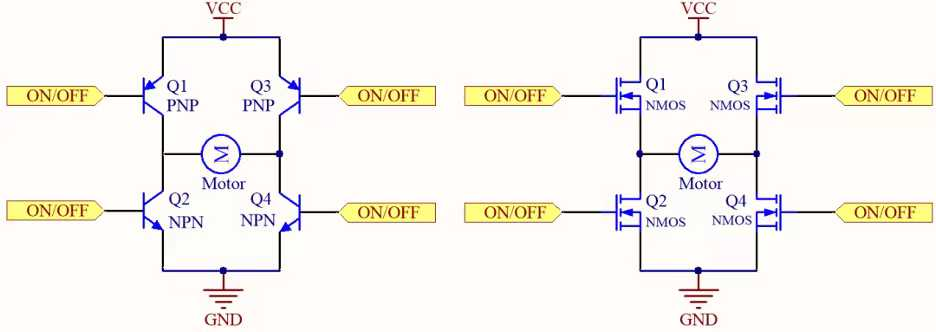
\includegraphics[width=0.8\textwidth]{../Photos/motor_theory}
  \caption{Two theories of motor}
  \label{fig:two-theories-of-motor}
\end{figure}

In figure~\ref{fig:pulse_width_modulation}, the duty cycle refers to the average rate within a period. 
The rotation speed of the motor can be controlled based on the ratio of the high-level voltage to the low-level voltage within the period.
\begin{figure}[H]
  \centering
  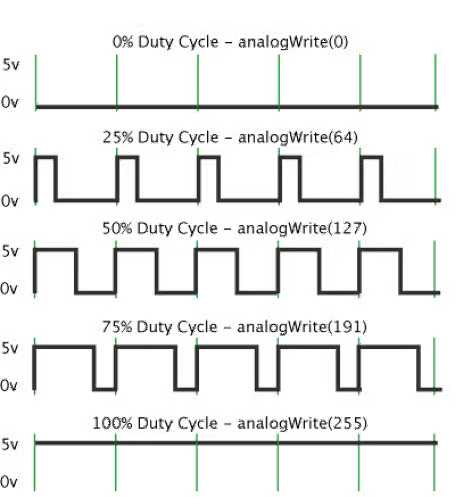
\includegraphics[width=0.5\textwidth]{../Photos/Pulse_Width_Modulation}
  \caption{Pulse Width Modulation}
  \label{fig:pulse_width_modulation}
\end{figure}


\section*{Methods}
% Describe the technical procedures to collect the results.
% Add figures into this section, where
% each figure and each equation may reduce the number of words you use.
\begin{table}[H]
  \centering
  \setlength{\arrayrulewidth}{1pt}
  \begin{tabularx}{0.8\textwidth}{@{\hspace{35pt}}cl}
    \hline
    abridge & \multicolumn{1}{c}{full name} \\
    \hline
    \textbf{ADC} & Analog-to-Digital Conversion \\
    \textbf{IDE} & Integrated Development Environment \\
    \textbf{DC motor} & direct current motor \\
    \hline
  \end{tabularx}
\end{table}

\subsection*{Experiment 1: Constructing a Circuit to Control a Motor Using chip L293D}
\label{sub:experiment-1}
Utilizing the built-in H-bridge circuit of the L293D chip, as figure~\ref{fig:l293d} shows, 
precise control of the motor's rotation direction can be achieved by manipulating the voltage state of the Enable Pin 1 and the output pins 1 (out1) and 2 (out2). 
Specifically, when Enable Pin 1 is at a low voltage level, the motor will not rotate. 
Conversely, when Enable Pin 1 is at a high voltage level, 
if output pin 1 (out1) is at a high voltage and output pin 2 (out2) is at a low voltage, the motor will rotate clockwise. 
On the other hand, if output pin 1 (out1) is at a low voltage and output pin 2 (out2) is at a high voltage, the motor will rotate counterclockwise.
\begin{figure}[H]
    \centering
    \begin{subfigure}{0.45\textwidth}
        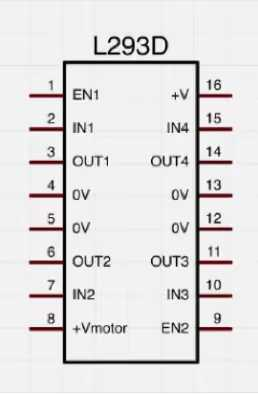
\includegraphics[angle=90, width=0.8\linewidth]{../Photos/L293D}
    \end{subfigure}
    \hfill
    \begin{subfigure}{0.45\textwidth}
        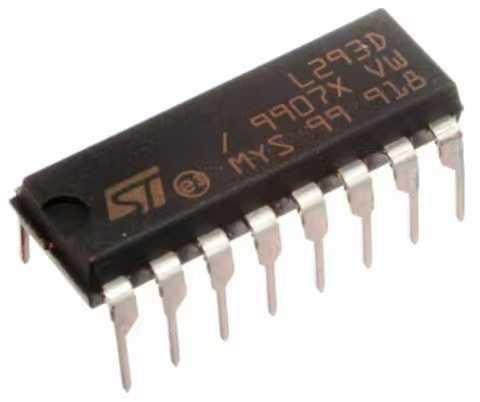
\includegraphics[width=0.6\linewidth]{../Photos/L293D_real}
    \end{subfigure}
    \caption{L293D}
    \label{fig:l293d}
\end{figure}

Based on the chip \textit{L293D}, we built the following circuit and the in figure~\ref{fig:basic-circuit}:
\begin{figure}[H]
  \centering
  \begin{subfigure}{0.45\textwidth}
    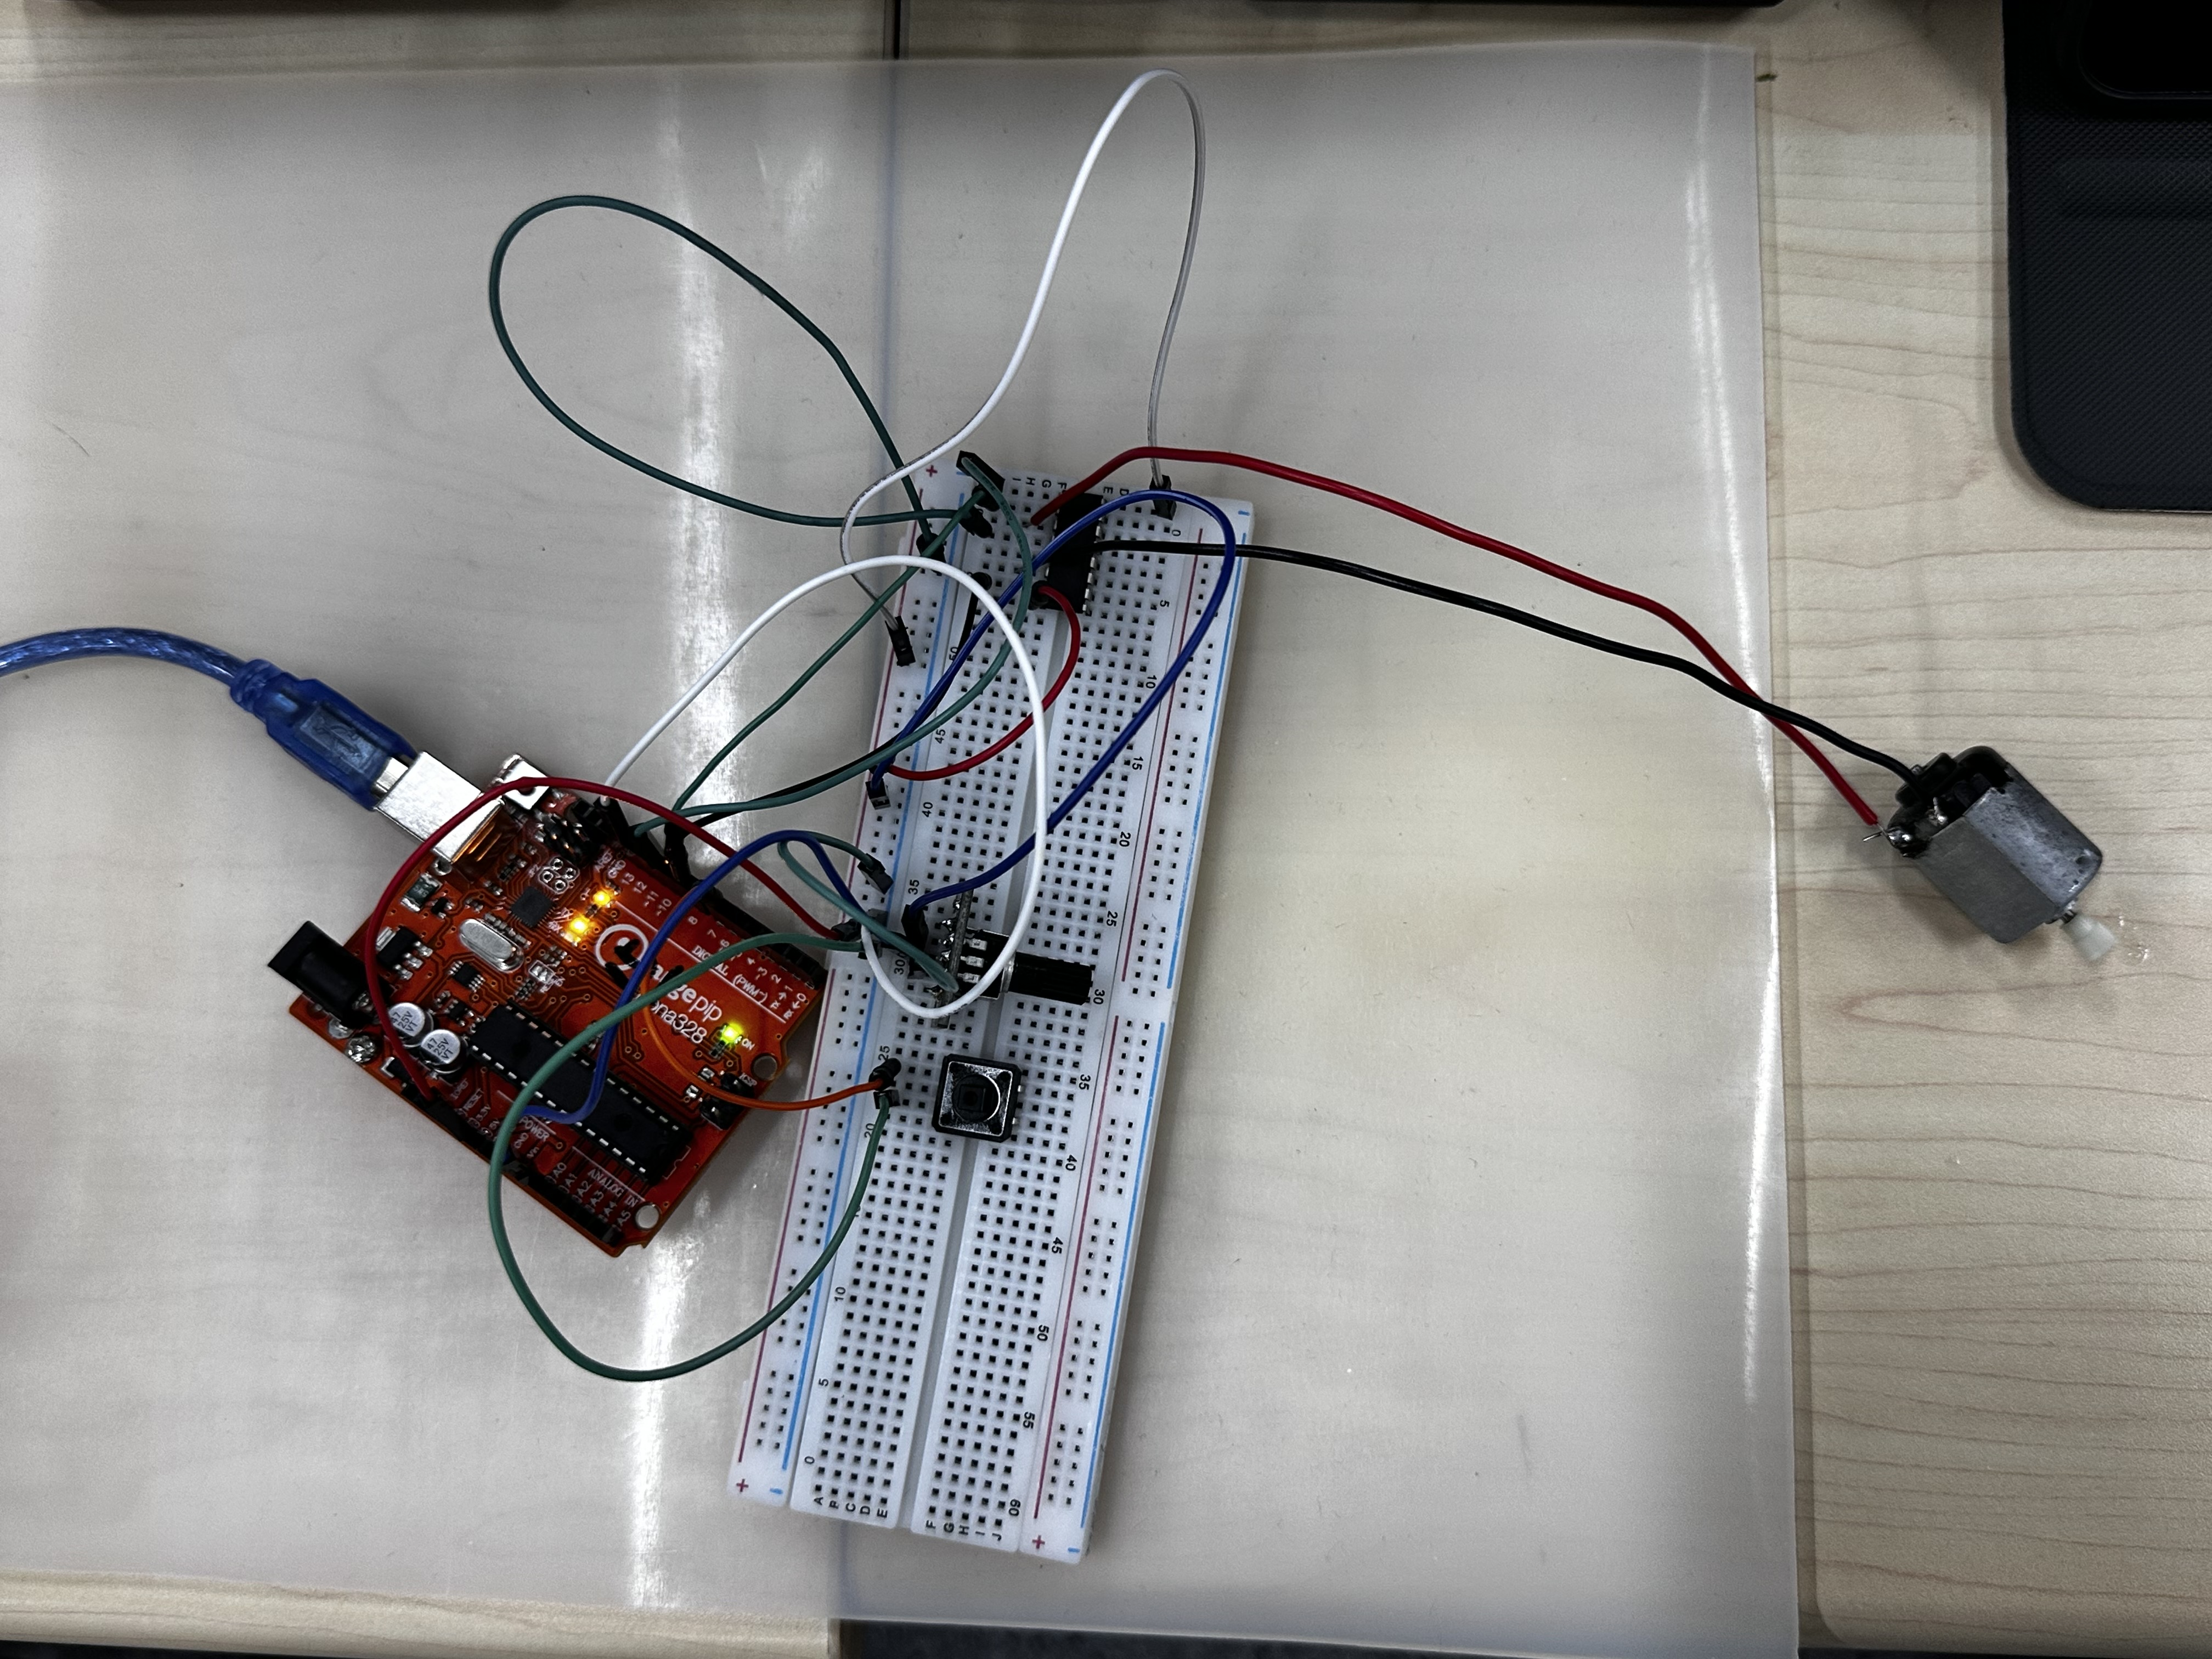
\includegraphics[width=0.7\linewidth]{../Photos/Connection/actual/Motor_actual_1}
  \end{subfigure}
  \hfill
  \begin{subfigure}{0.45\textwidth}
    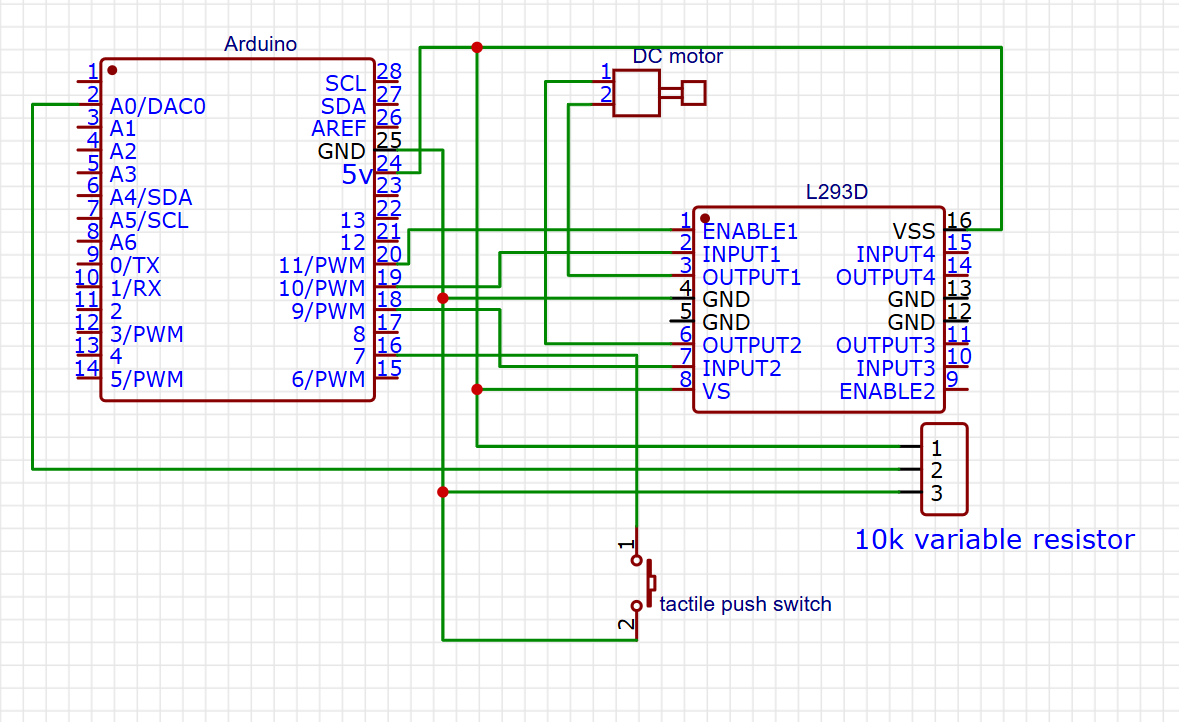
\includegraphics[width=0.8\linewidth]{../Photos/Connection/JLC/Motor_JLC_1}
  \end{subfigure}
  \caption{Basic Circuit}
  \label{fig:basic-circuit}
\end{figure}

\subsection*{Experiment 2: Measuring the Range of Motor Speed Variation with Different PWM Values and Changes in the Resistance of the Potentiometer}
To quantitatively analyze the relationship between the resistance of a variable resistor and the rotation speed of a motor, 
we employed an indirect measurement method. 
Specifically, we connected a fixed-value resistor in series with the variable resistor and measured the voltage across this fixed-value resistor. 
By doing so, we were able to calculate the voltage and current applied across the variable resistor, 
thereby accurately determining its resistance value. 
This approach effectively enabled a quantitative analysis of the variable resistor's resistance and 
provided reliable data support for studying its relationship with the motor's rotation speed.
These are showed in figure~\ref{fig:advanced-circuit}.
\begin{figure}[H]
  \centering
  \begin{subfigure}{0.45\textwidth}
    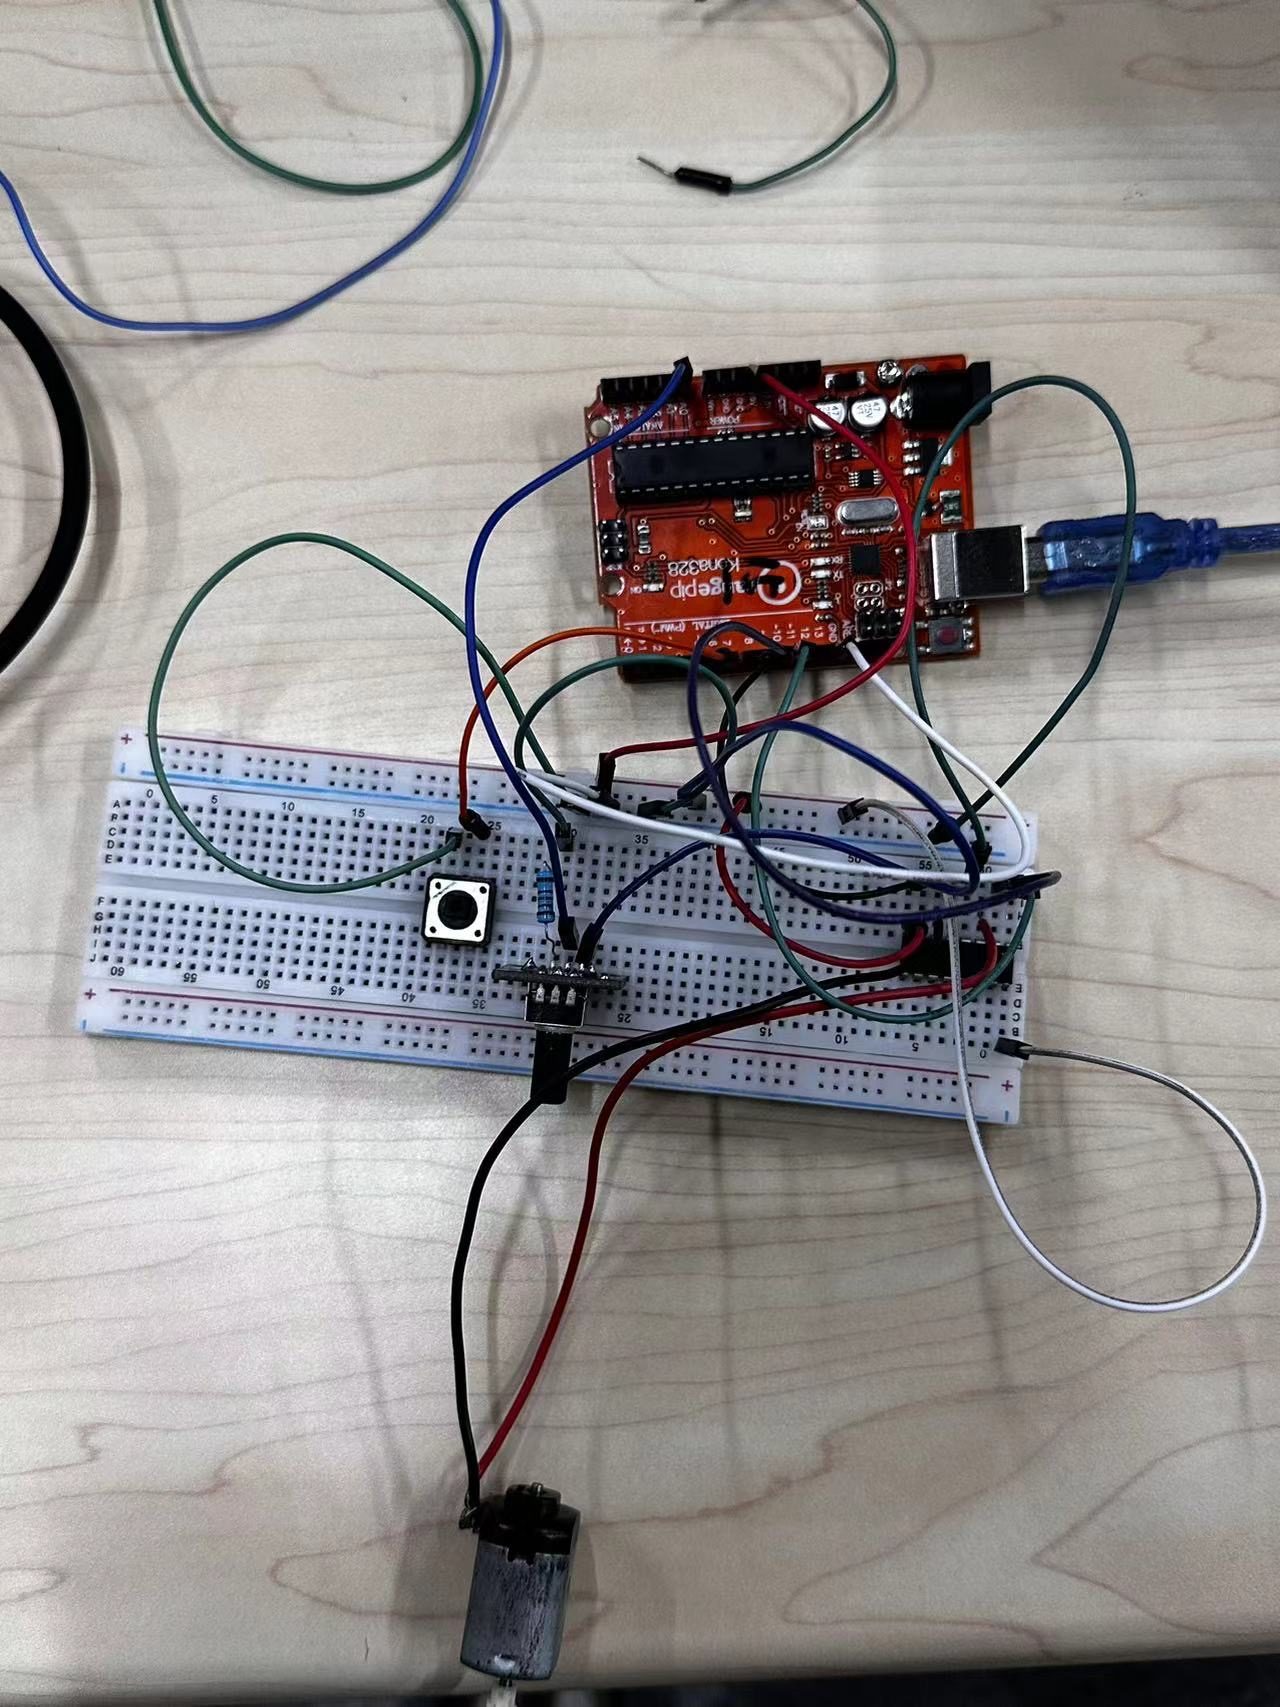
\includegraphics[angle=90, width=0.7\linewidth]{../Photos/Connection/actual/Motor2R_actual_1}
  \end{subfigure}
  \hfill
  \begin{subfigure}{0.45\textwidth}
    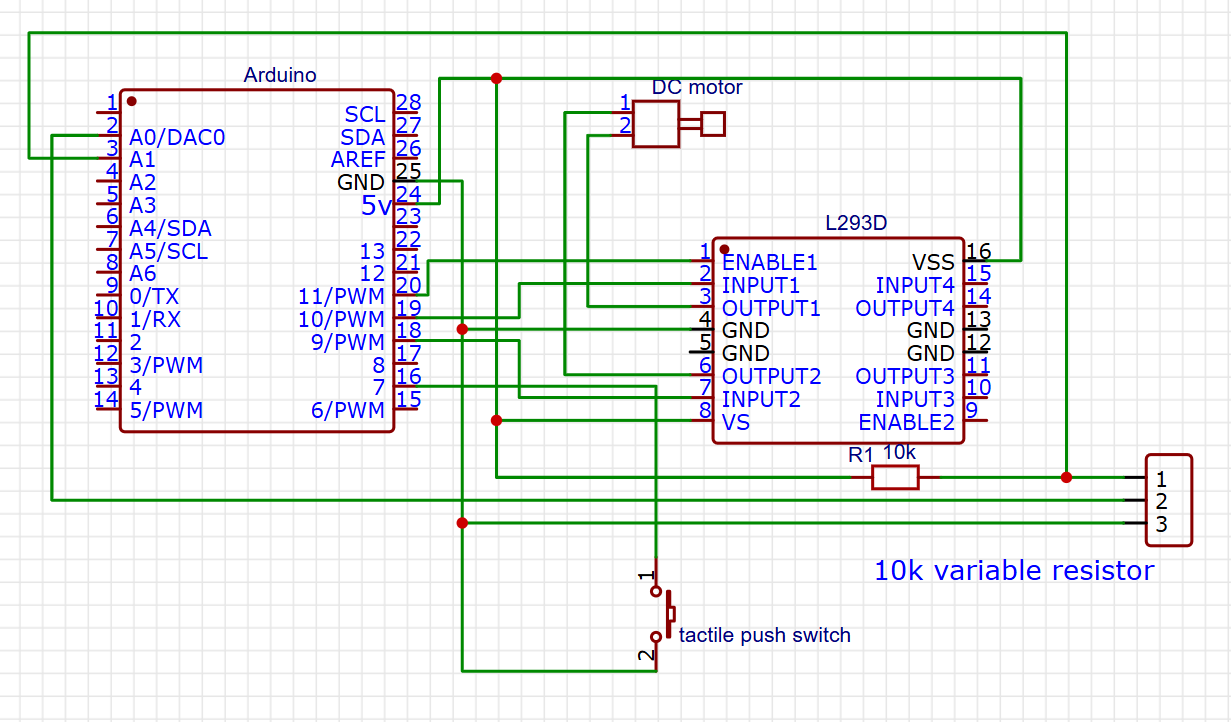
\includegraphics[width=0.8\linewidth]{../Photos/Connection/JLC/Motor2R_JLC_1}
  \end{subfigure}
  \caption{Advansed Circuit}
  \label{fig:advanced-circuit}
\end{figure}

The purpose of this experiment is to obtain the real-time rotational speed of the motor and to calculate the resistance value of the potentiometer through voltage division by connecting a fixed resistor in series. 
It can be further divided into four sub-experiments with PWM values of full, 3/4, 2/4, and 1/4.
Formulas are based on follows:
\begin{equation}
  Voltage = \frac{V_{A_0}}{1023} \times V_{ref}
\end{equation}
\begin{equation}
  V_{out} = V_{ref} \times \frac{R_{pot}}{R_{pot} + R_{fixed}}
\end{equation}
\begin{equation}
  R_{pot} = R_{fixed} \times \frac{V_{CC} - V_{out}}{V_{out}}
\end{equation}

The real-time speed and the corresponding resistance value of the potentiometer are obtained by dividing the value after analog-to-digital conversion (ADC) of the voltage on analog pin A0, 
acquired through the IDE's Serial Monitor, by 4.

\subsection*{Experiment 3: Controlling the Forward and Reverse Rotation of the Motor}
This experiment aims to control the forward and reverse rotation of the motor by using an H-bridge to change the high/low voltage levels of \textit{IN1} and \textit{IN2}. 
The implementation method is the same as in Experiment 1~\ref{sub:experiment-1}, so it will not be elaborated further here.

The program is written using Arduino IDE to obtain the voltage values from the analog pins A0 and A1.

\section*{Results}
% Add all appropriate figures and analysis.
% No formal word count for this section, however
% please keep text as concise as possible.
\subsection*{Experiment 1:}
We have successfully constructed a circuit containing the L293D to control the rotation of a motor (including stopping, rotating, changing speed, and changing the direction of rotation).

\subsection*{Experiment 2:}
We obtained the voltage value on analog pin A0 after analog-to-digital conversion (ADC) through the Serial Monitor in the IDE. 
By dividing this value by 4, 
we calculated the real-time rotational speed and the corresponding resistance value of the sliding rheostat. 
The specific details are as follows:
\begin{itemize}
  \item \textbf{4/4 PWM}

  \textcolor{gray}{speed: [ 136, 136, 134, 135, 135, 135, 137, 144, 153, 155, 160, 163, 166, 169, 174, 176, 179, 182, 183, 184, 185, 187, 188, 190, 191, 193, 194, 196, 197, 196, 196, 198, 198, 200, 200, 202, 202, 203, 202, 205, 206, 206, 209, 208, 209, 211, 216, 216, 214, 213, 216, 214, 216 ]}

  \textcolor{gray}{pot\_lin: [ 527, 527, 524, 525, 525, 524, 532, 564, 597, 611, 629, 635, 641, 651, 669, 671, 691, 699, 693, 707, 715, 723, 720, 735, 743, 748, 748, 751, 767, 760, 770, 778, 787, 782, 801, 802, 805, 808, 813, 822, 816, 825, 823, 844, 847, 851, 862, 866, 868, 865, 863, 861, 856 ]}
  \begin{figure}[H]
    \centering
    \includegraphics[width=0.8\textwidth]{../Photos/Chart/424_MOTOR_CLOCKWISE}
  \end{figure} 

  \item \textbf{3/4 PWM}

  \textcolor{gray}{speed: [ 100, 100, 100, 99, 100, 105, 110, 114, 117, 121, 123, 126, 128, 129, 132, 133, 135, 136, 137, 140, 141, 143, 144, 146, 148, 150, 150, 152, 153, 155, 156, 157, 158, 159, 161, 162, 162, 163, 162, 162, 159, 159, 160 ]}

  \textcolor{gray}{pot\_lin: [ 522, 520, 520, 520, 521, 547, 576, 602, 620, 637, 649, 661, 676, 681, 695, 703, 707, 711, 714, 725, 730, 739, 745, 750, 759, 770, 770, 773, 790, 804, 802, 815, 820, 828, 835, 844, 851, 858, 858, 858, 844, 845, 850 ]}
  \begin{figure}[H]
    \centering
    \includegraphics[width=0.8\textwidth]{../Photos/Chart/324_MOTOR_CLOCKWISE}
  \end{figure} 

  \item \textbf{2/4 PWM}

  \textcolor{gray}{speed: [ 53, 57, 54, 57, 58, 60, 61, 63, 63, 63, 69, 72, 75, 79, 81, 82, 85, 87, 89, 91, 93, 95, 96, 97, 99, 101, 102, 102, 104, 104, 105, 106, 107, 108, 109, 109, 109, 109, 109, 110, 110, 109, 108 ]}

  \textcolor{gray}{pot\_lin: [ 539, 529, 542, 538, 533, 552, 419, 416, 403, 395, 441, 467, 499, 532, 565, 578, 601, 620, 639, 655, 675, 695, 707, 725, 743, 750, 751, 759, 765, 767, 775, 781, 786, 795, 799, 805, 806, 806, 807, 805, 819, 837, 839 ]}
  \begin{figure}[H]
    \centering
    \includegraphics[width=0.8\textwidth]{../Photos/Chart/224_MOTOR_CLOCKWISE}
  \end{figure} 

  \item \textbf{1/4 PWM}

  \textcolor{gray}{speed: [ 31, 31, 31, 31, 31, 33, 34, 36, 37, 38, 39, 40, 41, 42, 43, 44, 45, 46, 47, 47, 48, 49, 50, 50, 51, 51, 52, 53, 53, 54, 54, 55, 55, 54, 54, 54 ]}

  \textcolor{gray}{pot\_lin: [ 450, 462, 474, 490, 508, 531, 559, 580, 602, 614, 630, 646, 665, 684, 698, 715, 724, 736, 750, 762, 775, 785, 797, 806, 816, 825, 836, 844, 853, 861, 870, 875, 876, 861, 863, 870 ]}
  \begin{figure}[H]
    \centering
    \includegraphics[width=0.8\textwidth]{../Photos/Chart/124_MOTOR_CLOCKWISE}
  \end{figure} 
\end{itemize}

\subsection*{Experiment 3:}
The corresponding parameter is obtained through the IDE's Serial Monitor as follows:
\begin{verbatim}
Clockwise: 
Speed: 136; Sequence: Clockwise; POT-LIN: 527
Speed: 136; Sequence: Clockwise; POT-LIN: 527
Speed: 134; Sequence: Clockwise; POT-LIN: 524
...

Counter-Clockwise: 
Speed: 132; Sequence: Counter-Clockwise; POT-LIN: 526
Speed: 136; Sequence: Counter-Clockwise; POT-LIN: 526
Speed: 135; Sequence: Counter-Clockwise; POT-LIN: 525
...
\end{verbatim}

\section*{Conclusions}
% Please give the conclusions from the characterisations including a summary of the results collected.
\subsection*{Summary}
This experiment can be devided into three sub-experiments:
\begin{itemize}
  \item \textbf{Using the L293D Chip to Drive a DC Motor:} 
  We successfully utilized the L293D chip to control the rotation of a DC motor, 
  including starting, stopping, and changing the speed and direction of rotation.
  \item \textbf{Measuring Motor Speed Under Different PWM Conditions:} 
  We investigated how the motor speed varied with voltage changes under different PWM (Pulse Width Modulation) settings. 
  Since the resistance of the sliding rheostat cannot be measured directly, 
  we connected a 10 kΩ resistor in series to indirectly measure the voltage and thereby calculate the motor speed.
  \item \textbf{Controlling Motor Direction with an H-Bridge:} 
  By manipulating the voltage levels at the IN1 and IN2 terminals of the H-bridge, 
  we were able to control the direction of the motor, 
  enabling it to rotate either clockwise or counterclockwise.
\end{itemize}
Through these experiments, 
we have gained a thorough understanding of the principles of the H-bridge and the control of DC motors. 
This knowledge will serve as a solid foundation for our future projects, 
such as controlling the speed and direction of a small vehicle's wheels.

\subsection*{Limitations}
1. The range of the sliding rheostat used in this experiment is unknown. 
Moreover, the resistance cannot be manually controlled to change linearly, 
which may introduce certain experimental errors.

2. The rotor of the motor used in this experiment has some sticking issues, 
which may lead to deviations when we visually observe and record the motor’s rotation.

\newpage
\section*{Appendix}
\begin{itemize}
  \item The code of \textbf{Arduino IDE} to gain data is as follows:\\
  \begin{lstlisting}[language=C++]
int enablePin = 11;
int in1Pin = 10;
int in2Pin = 9;
int switchPin = 7;
int potPin = 0;
int fixedR = 10000;
int VCC = 5;

void setup() {
  // put your setup code here, to run once:
  pinMode(in1Pin, OUTPUT);
  pinMode(in2Pin, OUTPUT);
  pinMode(enablePin, OUTPUT);
  pinMode(switchPin, INPUT_PULLUP);
  Serial.begin(9600);
}

void loop() {
  // put your main code here, to run repeatedly:
  int speed = (analogRead(potPin) / 4) * 1 / 4;
  Serial.print("Speed: ");
  Serial.print(speed);
  Serial.print(";\t");

  boolean reverse = digitalRead(switchPin);
  Serial.print("Sequence: ");

  if(reverse == 1) {
    Serial.print("Clockwise");
  } else {
    Serial.print("Counter-Clockwise");
  }
  Serial.print(";\t");

  setMotor(speed, reverse);

  int sensorValue_A0 = analogRead(A0);
  float Vout = (sensorValue_A0 / 1023.0) * VCC;
  float Rpot = fixedR * ((VCC - Vout) / Vout);
  Serial.print("POT-LIN: ");
  Serial.println(sensorValue_A0);

  delay(1);
  delay(500);
}

void setMotor(int speed, boolean reverse) {
  analogWrite(enablePin, speed);
  digitalWrite(in1Pin, !reverse);
  digitalWrite(in2Pin, reverse);
}
  \end{lstlisting}
  
  \item The code of \textbf{Python} to process data and generate charts is as follows:
  \begin{lstlisting}[language=Python]
import numpy as np
import mlx.core as mx
import matplotlib.pyplot as plt

speed =  [
    136, 136, 134, 135, 135, 135, 137, 144, 153, 155, 160, 163, 166, 169, 174,
    176, 179, 182, 183, 184, 185, 187, 188, 190, 191, 193, 194, 196, 197, 196,
    196, 198, 198, 200, 200, 202, 202, 203, 202, 205, 206, 206, 209, 208, 209,
    211, 216, 216, 214, 213, 216, 214, 216
]
pot_lin = [
    527, 527, 524, 525, 525, 524, 532, 564, 597, 611, 629, 635, 641, 651, 669,
    671, 691, 699, 693, 707, 715, 723, 720, 735, 743, 748, 748, 751, 767, 760,
    770, 778, 787, 782, 801, 802, 805, 808, 813, 822, 816, 825, 823, 844, 847,
    851, 862, 866, 868, 865, 863, 861, 856
]

speed = mx.array(speed)
pot_lin = mx.array(pot_lin)

poly_degree = 6
poly_coeffs = np.polyfit(speed, pot_lin, poly_degree)
poly_func = np.poly1d(poly_coeffs)

speed_dense = mx.linspace(speed.min(), speed.max(), 300)
pot_lin_dense = poly_func(speed_dense)

plt.figure(figsize=(10, 6))
plt.plot(speed, pot_lin, 'ro', label='Original Data')
plt.plot(speed_dense, pot_lin_dense, 'b-', label=f"Fitting Curve (Degree-{poly_degree})")

plt.xlabel("Speed")
plt.ylabel(r"POT-LIN / $\Omega$")
plt.title('Speed - POT-LIN (4/4 PWM)')
plt.grid(True)
plt.legend()

plt.savefig("./Photos/Chart/424_MOTOR_CLOCKWISE.png", dpi=1200)
  \end{lstlisting}
\end{itemize}

\end{document}